%%%%%%%%%%%%%%%%%%%%%%%%%%% asme2e.tex %%%%%%%%%%%%%%%%%%%%%%%%%%%%%%%
% Template for producing TSFP-format articles using LaTeX
% Based on the asme2e template (http://iel.ucdavis.edu/code/ASME/)
% Modified: 11 February 2013 for TSFP8 by R. Manceau
% Modified: 05 May 2014 for TSFP9&10 by K. Chauhan
% In case of problem: kapil.chauhan@sydney.edu.au
%%%%%%%%%%%%%%%%%%%%%%%%%%%%%%%%%%%%%%%%%%%%%%%%%%%%%%%%%%%%%%%%%%%%%%

%%%%%%%%%%%%%%%%%%%%%%%%%%%%%%%%%%%%%%%%%%%%%%
% To generate a pdf, compile either with pdflatex
% or with latex and
% dvips tsfp_template -Ppdf -t a4 -o
% followed by
% ps2pdf tsfp_template.ps
% (avoid using dvipdf that does not preserve the page layout on some systems)
%%%%%%%%%%%%%%%%%%%%%%%%%%%%%%%%%%%%%%%%%%%%%%

%%% use twocolumn and 10pt options with the tsfp format
\documentclass[twocolumn,10pt]{tsfp}
\usepackage{flushend}
\usepackage{graphicx}
%\usepackage{color}
\usepackage{amssymb}
\usepackage{amsmath}
\usepackage{amssymb}
\usepackage[authoryear,round]{natbib}
\usepackage{subcaption}
\usepackage{placeins}
\usepackage[usenames, dvipsnames]{color}

\definecolor{mygray}{gray}{0.4}

\title{UNSTEADY AERODYNAMIC EFFECTS IN PITCHING AIRFOILS STUDIED THROUGH LARGE-EDDY SIMULATIONS}

%%%% In case you need to slightly adapt the horizontal spacing between authors (for more than 3 authors) uncomment the following command
%%%% and if necessary modify the factor
%\renewcommand{\expauthors}{1.1}

%%% first author
\author{Prabal S. Negi
	\affiliation{
		Linn\'e FLOW Centre, KTH Mechanics\\
		SE-100 44 Stockholm, Sweden\\
		negi@mech.kth.se
	}
}

%%% second author
%%% remove the following entry for single author papers
%%% add more entries for additional authors
\author{Ricardo Vinuesa
	\affiliation{
		Linn\'e FLOW Centre, KTH Mechanics\\
		SE-100 44 Stockholm, Sweden\\
		rvinuesa@mech.kth.se
	}
}

\author{Philipp Schlatter
	\affiliation{
		Linn\'e FLOW Centre, KTH Mechanics\\
		SE-100 44 Stockholm, Sweden\\
		pschlatt@mech.kth.se
	}
}

\author{Ardeshir Hanifi
	\affiliation{
		Linn\'e FLOW Centre, KTH Mechanics\\
		SE-100 44 Stockholm, Sweden\\
		ardeshir@mech.kth.se
	}
}

\author{Dan S. Henningson
	\affiliation{
		Linn\'e FLOW Centre, KTH Mechanics\\
		SE-100 44 Stockholm, Sweden\\
		henning@mech.kth.se
	}
}


\begin{document}

\maketitle   %Print title matter

% Set the font to 9pt.
\fontsize{9}{11}\selectfont

%%%%%%%%%%%%%%%%%%%%%%%%%%%%%%%%%%%%%%%%%%%%%%%%%%%%%%%%%%%%%%%%%%%%%%
\section*{ABSTRACT}

Wall-resolved large-eddy simulations (LES) are utilized to investigate the flow-physics of an airfoil undergoing pitch oscillations. A relaxation-term (RT) based filtering procedure is employed to add limited high order dissipation to account for the dissipation from the smallest scales which are not resolved. Validation of the procedure is presented for turbulent channel flows and for flow around a wing section. The procedure is then used for the simulation of small-amplitude pitching airfoil at $Re_{c}=100,000$ with a reduced frequency $k=0.5$. The investigation of the unsteady phenomenon is done in the context of a natural laminar flow airfoil, the performance of which depends critically on the suction side transition characteristics. The dynamic range of the pitch cycle sees the appearance, destabilization and disappearance of a laminar separation bubble at the leading edge. An abrupt change is seen in the lift coefficient, which is linked to a rapid movement of the transition point over the suction side. Destabilization of the laminar separation bubble is the cause of these rapid transition movements which occur near the end of the pitch-up phase of the cycle.

%%%%%%%%%%%%%%%%%%%%%%%%%%%%%%%%%%%%%%%%%%%%%%%%%%%%%%%%%%%%%%%%%%%%%%

\FloatBarrier

\section*{INTRODUCTION}

A large focus of the studies on flow over pitching wings tends towards large pitch amplitudes and stall dynamics, with early experimental work by \cite{mccroskey82experimental} and \cite{carr1977} providing much of the initial understanding about the phenomenon. More recent works by \cite{dunne2015}, \cite{rival2010}, \cite{choudhry14} \emph{etc.} continue the investigation of the process. The review by \cite{mccroskey82} and a more recent one by \cite{coorke15} provide an overview of the development of unsteady airfoil behavior. Much lesser attention has gone towards studying unsteady aerodynamic behavior in the cases of small pitch amplitudes. Some works dealing with small pitch amplitudes include the work done by \cite{pascazio96} which shows a time delay in laminar-turbulent transition during pitching. \cite{nati15} study the effect of small amplitude pitching on a laminar separation bubble at low Reynolds numbers. 
\begin{figure}[b]
	\centering
	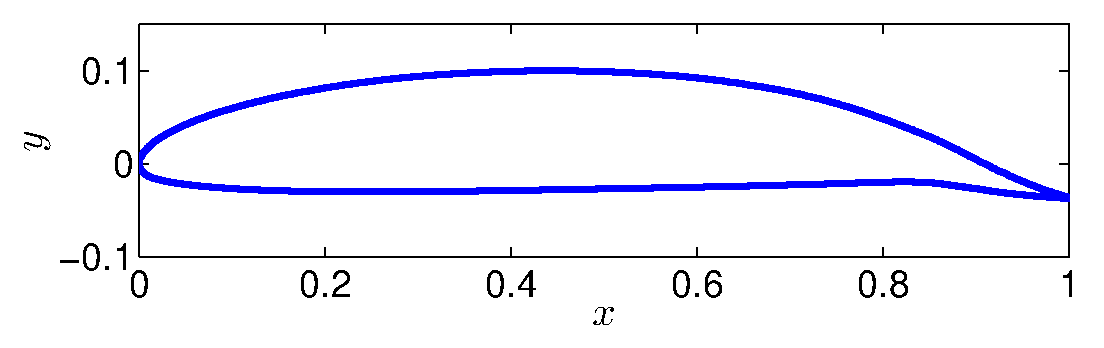
\includegraphics[width=0.9\columnwidth]{foil}
	\caption{Natural Laminar Flow (NLF) airfoil used in the current study.}
	\label{fig:foil_david}
\end{figure}
Such cases qualitatively represent small changes in operating conditions, such as structural deformations or small trailing edge flap deflections. The understanding of flow response to such changes can be crucial in cases where small perturbations induce large changes in aerodynamic forces. The aerodynamic performance of natural laminar flow (NLF) airfoils critically depends on maintaining laminar flow over the suction side of the airfoil and such airfoils can exhibit sensitive dependence on the transition location, \emph{viz.} the operating conditions. The current work investigates the effect of small pitch oscillations on one such laminar airfoil (figure~\ref{fig:foil_david}), which was designed at the Aeronautical and Vehicle Engineering department of KTH where the same airfoil has been used in some experimental and numerical works \citep{lokatt17}. The simulations were performed at ``off-design" conditions at a lower Reynolds number, where the above mentioned sensitivity to operating conditions is observed. Calculations using an integral boundary layer code, Xfoil, \cite{drela89}, predict sharp changes in the coefficient of moment ($C_{m}$) and suction side transition location (figure~\ref{fig:xfoil_cm}) above an angle of attack $\alpha>6^{\circ}$.
\begin{figure}[t]
	\centering
	\includegraphics[width=0.75\columnwidth]{cm-tr-xfoil}
	\caption{Coefficient of moment ($C_{m}$), displayed on the left axis, and suction side transition location, shown on the right axis. Values obtained using Xfoil.}
	\label{fig:xfoil_cm}
\end{figure}
In recent works, wall-resolved large-eddy simulations have proven to be an effective tool for studying flow physics at high Reynolds numbers but with a computational cost which is much lower than that of direct numerical simulations (DNS). Some of the works to utilize this method include spatially evolving boundary layers \citep{eitel14}, pipe flows \citep{chin15} and flow over wings \citep{uzun10} and \citep{lombard15}. Successful application of the approach has motivated the present work which aims to gain insight into the flow-physics of unsteady airfoils undergoing small amplitude pitch oscillations at a chord based Reynolds number of $Re_{c}=100,000$.
\begin{figure}[t]
	\centering
	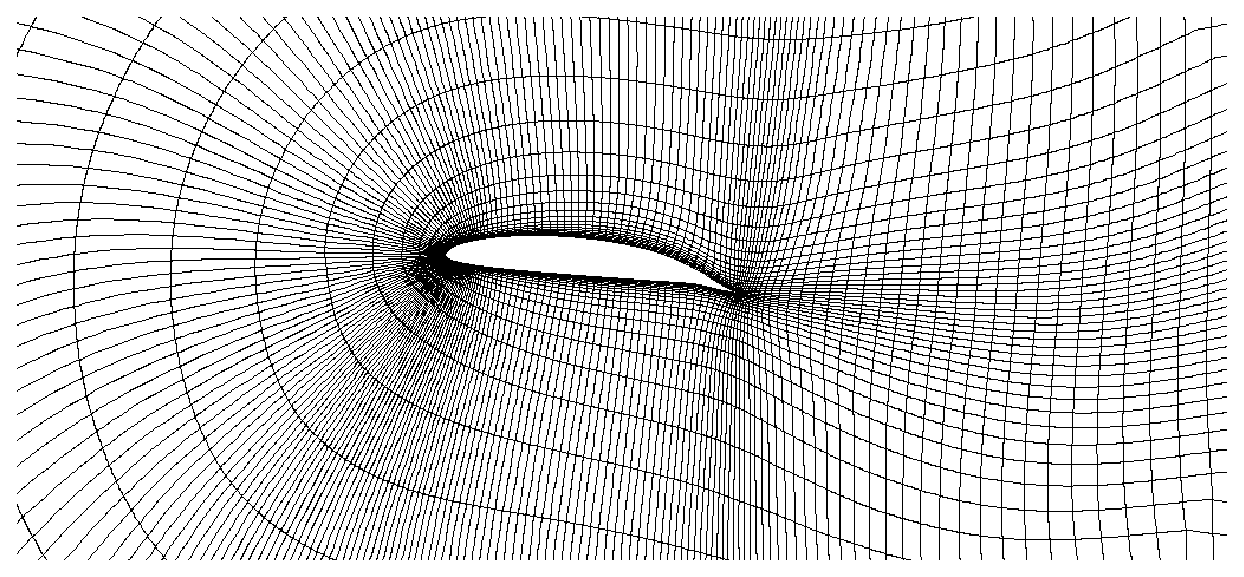
\includegraphics[width=0.9\columnwidth]{re100k_grid}
	\caption{Close-up of a 2D section of the spectral-element grid around the airfoil.}
	\label{fig:re100k_grid}
\end{figure}

\section*{NUMERICAL METHOD}

The computational code used for the simulations is Nek5000, which is an open source research code developed by \cite{nek5000} at Argonne National Laboratory. It is a based on a spectral-element method which allows the mapping of elements to complex geometries along with a high order spatial discretization within the elements. The method uses Lagrange interpolants of orthogonal Legendre polynomials as basis functions and utilizes Gauss--Lobatto--Legendre (GLL) quadrature for the distribution of points within the elements. The spatial discretization is done by means of the Galerkin approximation, following the $P_{N}-P_{N-2}$ formulation. An $11^{th}$ order polynomial interpolation is used within the spectral elements. The nonlinear terms are treated explicitly by third-order extrapolation (EXT3), whereas the viscous terms are treated implicitly by a third-order backward differentiation scheme (BDF3). Aliasing errors are removed with the use of over-integration. All equations are solved in non-dimensional units with the velocities normalized by the reference free-stream velocity $U_{0}$ and the length scales in all directions are normalized by the chord length $c$. The resultant non-dimensional time unit is given by $c/U_{0}$. Nek5000 is written in Fortran 77 and C with efficient scaling for up to 1 million MPI ranks. The simulations were carried out on the Cray XC40 system “Beskow” at the PDC Center at KTH in Stockholm (Sweden).
%%%%%%%%%%%%%%%%%%%%%%%%%%%%%%%%%%%%%%%%%%%%%%%%%%%%%%%%%%%%%%%%%%%%%%
\subsection*{RELAXATION-TERM LARGE-EDDY SIMULATION (RT-LES)}

The LES method is based on the ADM-RT approach first used by \cite{schlatter04}. The method supplements the governing equations with a dissipative term ($\chi\mathcal{H}(u)$). The equations of motion for the resolved velocity and pressure thus read:
\begin{eqnarray}
\frac{\partial u}{\partial t} + u\cdot\nabla u =  - \frac{1}{\rho}\nabla p + \frac{1}{Re}\nabla^{2}u -\chi\mathcal{H}(u) \\
\nabla\cdot u = 0
\end{eqnarray}
where $\mathcal{H}$ is a defined high-pass spectral filter and $\chi$ is a model parameter which together with $\mathcal{H}$ determines the strength of the dissipative term. The method has been used in earlier studies of boundary layer simulations in \cite{eitel14} and channel flows in \cite{schlatter06}, and has been shown to be reliable in predicting transition location and also preserving the characteristic structures which are seen in the DNS of transitional flows by \cite{schlatter06}.

\subsection*{COMPUTATIONAL SETUP}
A number of tests were carried out in a channel flow at a friction Reynolds number of $Re_{\tau}=395$, and the results are compared with the DNS data of \cite{moser99}. Finally the chosen resolution was set to $\Delta x^{+}=18$, $\Delta z^{+}=9$, with the first point in the wall-normal direction set at $\Delta y_{w}^{+}=0.64$ and the wall-normal resolution near the boundary layer edge is set to $y_{max}^{+}=12$. The superscript $^{+}$ indicates normalization in inner units. The resolution is very similar to the one used in \cite{eitel14} where the ADM-RT model is also used to simulate a spatially evolving boundary layer. A comparison of the results for the turbulent channel flow is shown for the mean velocity in figure~\ref{fig:vel_mean}, and for the turbulent kinetic energy budget (TKE) in figure~\ref{fig:budget}. The dissipation profile shown in the figure is the sum of resolved dissipation and the added dissipation by the relaxation term. A very good agreement with the DNS is found for the mean velocity and all the kinetic energy budget terms including the total dissipation.
\begin{figure}[t]
	\centering
	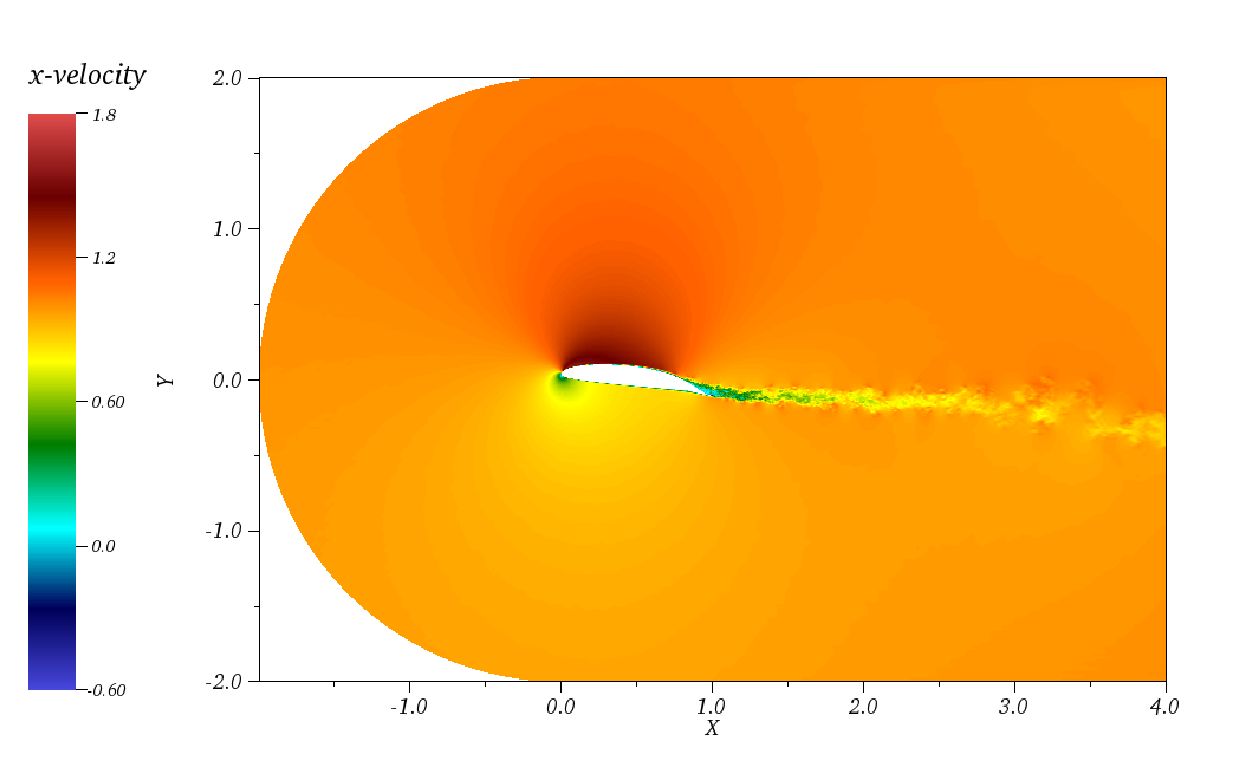
\includegraphics[width=1.0\columnwidth]{re100k_grid2}
	\caption{Simulation domain: Outflow boundary is $4$ chords downstream of the airfoil leading edge while the inflow boundary is $2$ chords away. Colored region represents a sectional view of the instantaneous streamwise velocity.}
	\label{fig:re100k_domain}
\end{figure}
\begin{figure}[t]
	\centering
	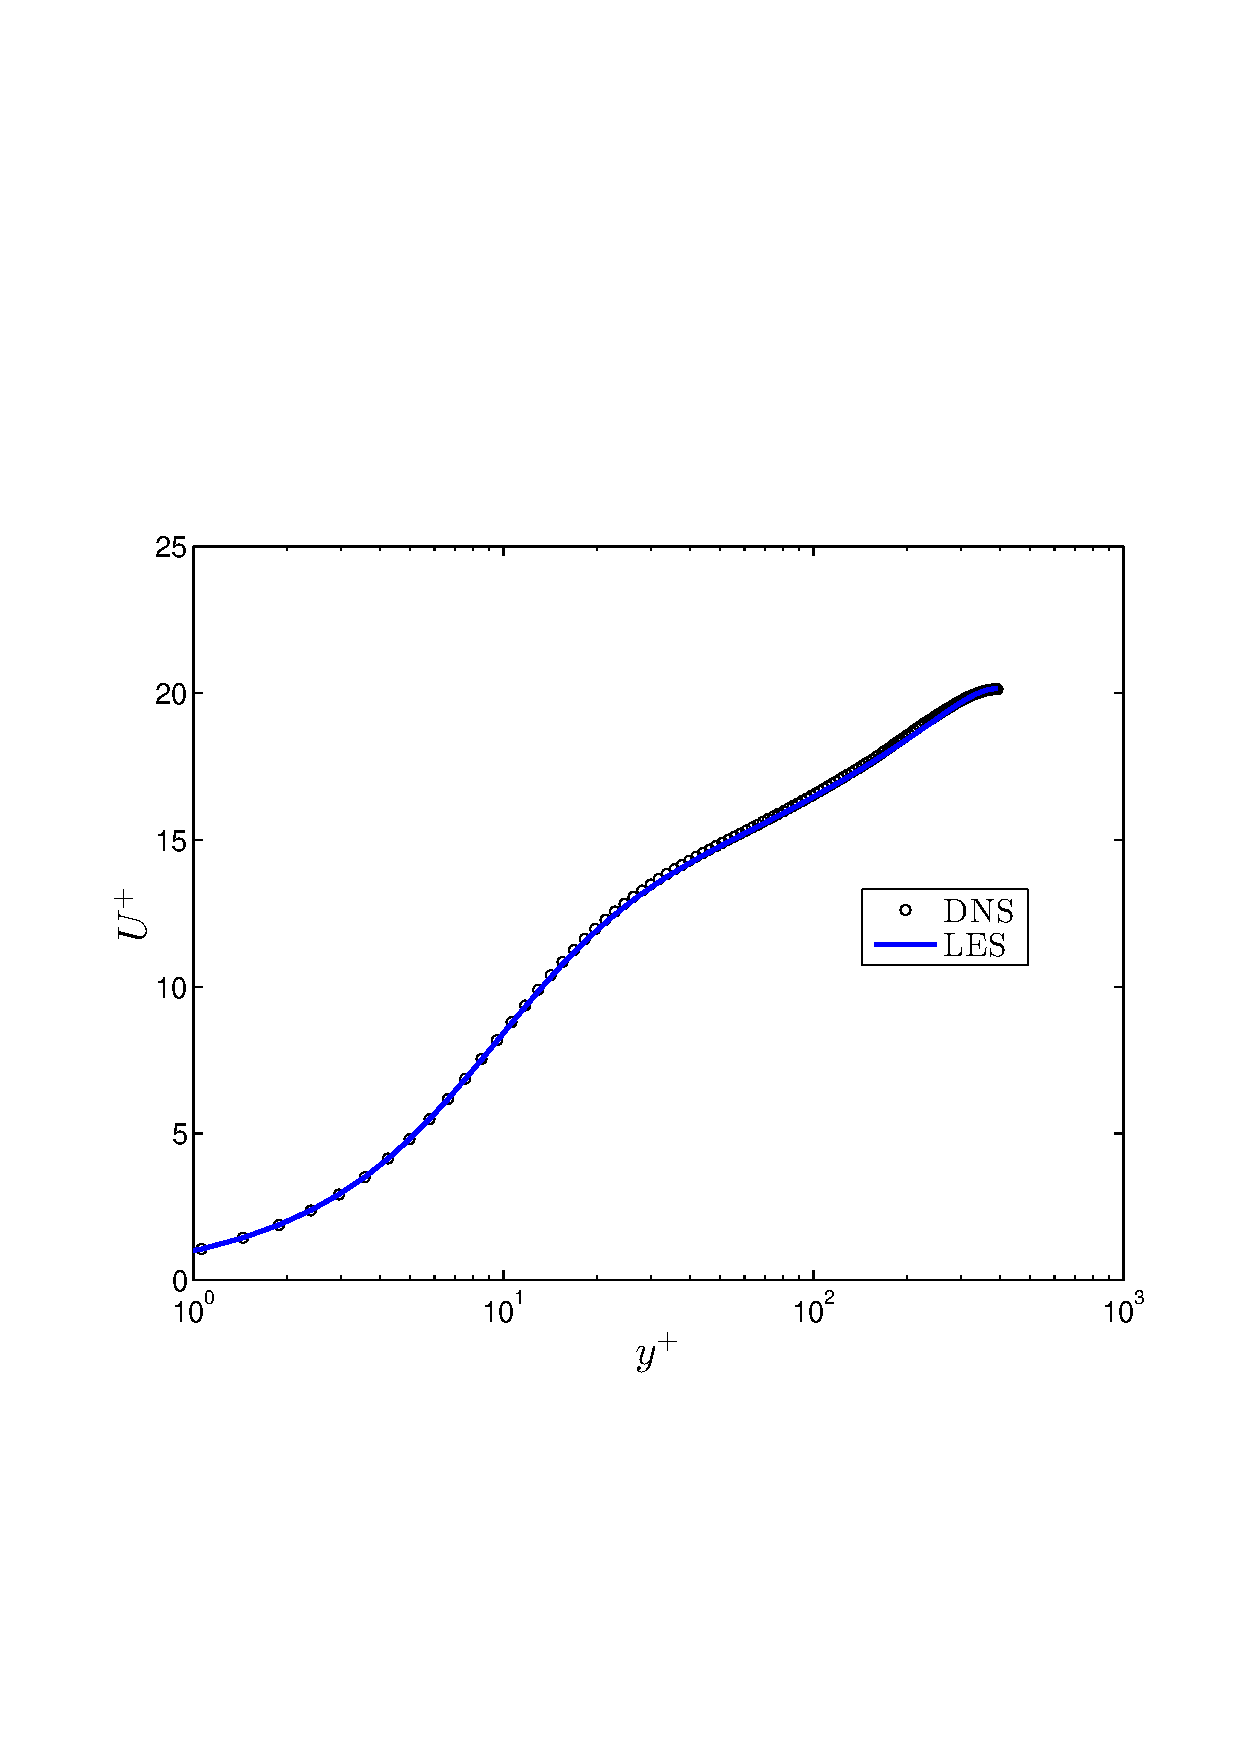
\includegraphics[width=0.8\columnwidth]{vel-log}
	\caption{Comparison of mean velocity profile normalized in inner units with DNS data from \cite{moser99}.}
	\label{fig:vel_mean}
\end{figure}
\begin{figure}[t]
	\centering
	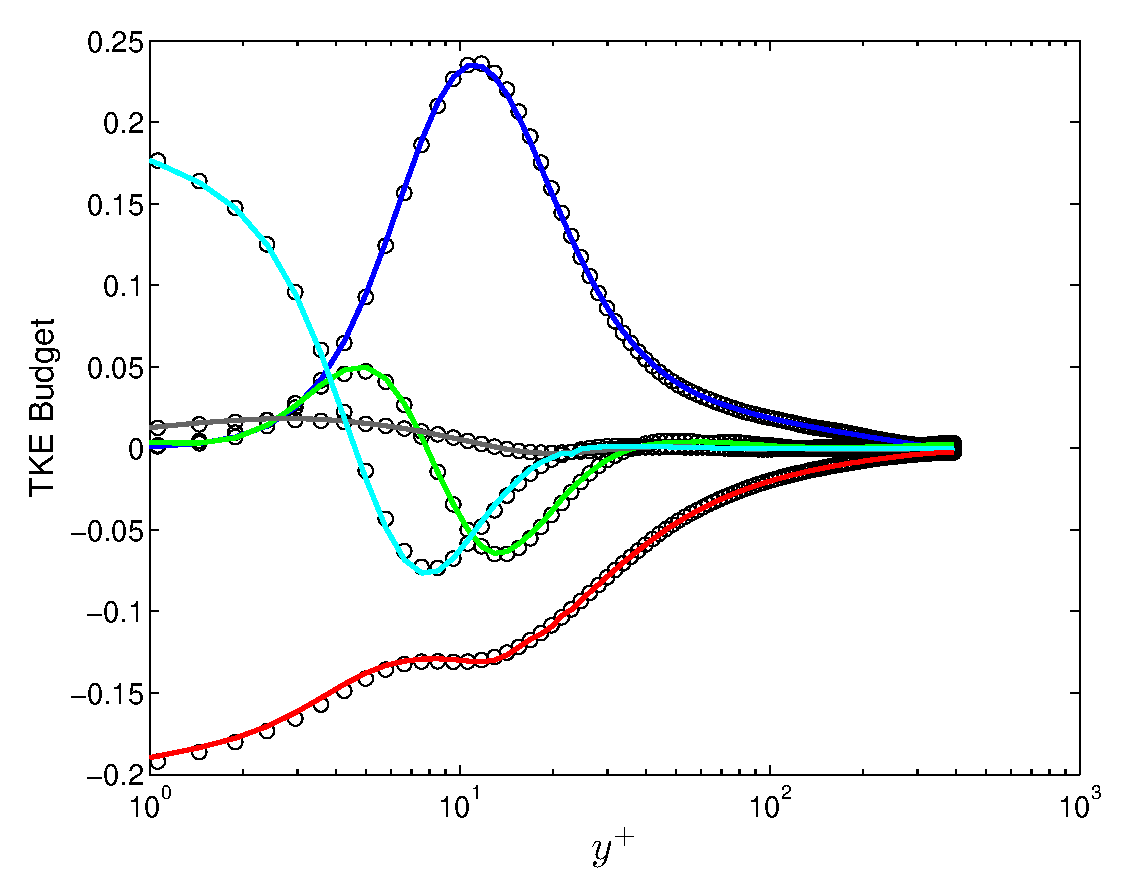
\includegraphics[width=0.8\columnwidth]{budgets}
	\caption{Comparison of turbulent kinetic energy budget normalized in inner units. Circles represent the DNS data from \cite{moser99} while the lines represent the values from the LES. The individual terms are color coded as: \textcolor{blue}{Production}, \textcolor{red}{Dissipation}, \textcolor{cyan}{Viscous diffusion}, \textcolor{green}{Turbulent diffusion}, \textcolor{mygray}{Velocity-Pressure correlation}}
	\label{fig:budget}
\end{figure}

The same resolution (in inner units) is then used to design the mesh around the airfoil, with additional care taken for special regions like the leading and trailing edge. Wall-shear stress data is obtained using Xfoil to estimate the grid spacing on the airfoil. A trip is introduced in Xfoil at $x/c\approx0.1$ to obtain turbulent wall-shear values on both the suction and pressure sides of the airfoil. Here $c$ denotes the chord length. Finally, the grid design uses the following criteria:

\begin{itemize}
	\item[$\bullet$] For $0.1<x/c<0.6$, $\Delta x^{+}=18$, $\Delta y_{wall}^{+}=0.64$ and $\Delta y_{max}^{+}=11$, using the local wall-shear ($\tau_{w}$) values on the airfoil. Since the flow is expected to be laminar on the pressure side, the stream-wise resolution is slightly relaxed to $\Delta x^{+}=25$ while keeping the same wall-normal resolution.
	\item[$\bullet$] For $x/c<0.1$, the peak $\tau_{w}$ value over the suction side of the airfoil is used to estimate the grid spacing.
	\item [$\bullet$] for $x/c>0.6$, the suction side experiences a large adverse pressure gradient which significantly reduces $\tau_{w}$ values. Therefore, the $\tau_{w}$ values from the pressure side are used for both the suction and pressure sides.
	\item [$\bullet$] A structured mesh is used, which is extruded in the span-wise direction. Hence the spanwise resolution is constant throughout the domain. The resolution is set to $\Delta z^{+}=9$, where the the peak $\tau_{w}$ value from the suction side is used.
\end{itemize}

A different criterion is needed for defining the resolution in the wake where the wall-based criteria do not hold. Accordingly, RANS simulations were performed using \textit{ANSYS}\textsuperscript{\textregistered} FLUENT, Academic Research, Release 16.1, to estimate the Kolmogorov length scale ($\eta$) in the wake region. The grid in the wake region is designed such that the average grid spacing between the GLL points follows the criteria: $\Delta x/\eta < 9$. A close-up of grid near the airfoil is shown in figure~\ref{fig:re100k_grid}. The far field boundaries are $2$ chords away from the airfoil leading edge in either direction and the outflow boundary is $4$ chords downstream from the airfoil leading edge. The inlet is designed as a curved inflow boundary with a constant radial distance of $2$ chords from the leading edge of the airfoil. The computational domain is $0.25$ chords wide in the spanwise direction. The domain can be visualized in figure~\ref{fig:re100k_domain}. The spectral-elements can be visualized in the close-up view (figure~\ref{fig:re100k_grid}). Each of the spectral-elements are further discretized by $12\times12\times12$ grid points in 3D, corresponding to an $11^{th}$ order spectral discretization. Periodic boundary conditions are imposed on the spanwise boundaries, while the outflow condition suggested by \cite{dong2014} is imposed on the outflow boundary. This outflow condition was shown to be accurate and stable in flows with strong back-flow velocities at the outflow boundary by \cite{dong2014}. Velocity field data is extracted from an unsteady RANS simulation and the time-averaged value is interpolated onto the domain inlet and far-field boundaries. The interpolated data is then imposed as a Dirichlet boundary condition on these boundaries. The method is very similar to the one used by \cite{hosseini16} in their DNS of flow around a wing section. In order to simulate low turbulence flight conditions, free-stream turbulence of intensity $Ti=0.1\%$ is superimposed on the Dirichlet boundary conditions. The free-stream turbulence is generated using Fourier modes with a von K\'arm\'an spectrum. The procedure is similar to the one described in \cite{brandt04} and has been used for the study of transition in flat plate boundary layers under the influence of free-stream turbulence.

A validation of the above criterion for complex geometries such as a wing section was performed at a chord based Reynolds number of $Re_{c}=400,000$ for NACA4412 airfoil. The LES grid resolution was setup with the same grid criteria as described above. The domain boundaries and boundary conditions are identical to the setup in \cite{hosseini16}. The results are validated using the DNS data from \cite{hosseini16}. Wall-normal profiles of the normalized kinetic energy budget is shown in figure~\ref{fig:wing_budget}. The profiles are extracted a streamwise location of $x/c=0.7$ on the suction side of the airfoil. The LES profiles (lines) match very well with the DNS data (circles), signifying the high accuracy of the LES with the current resolution.
\begin{figure}[h]
	\centering
	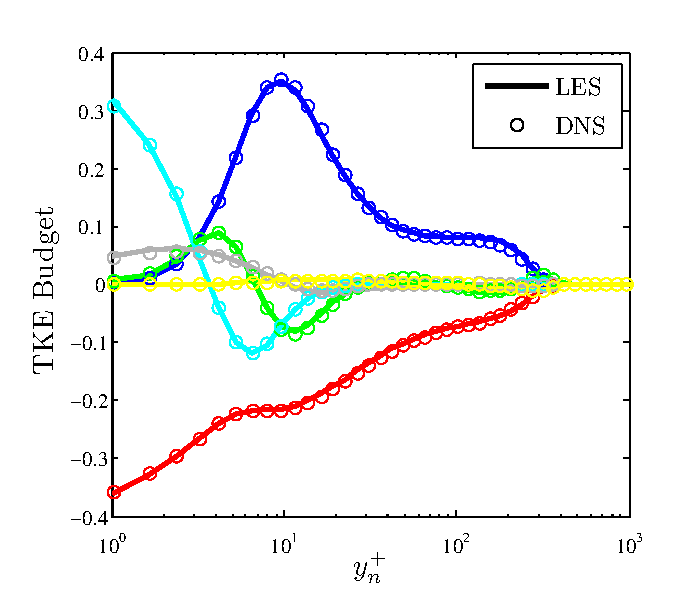
\includegraphics[width=0.85\columnwidth]{tke_vs_yp.pdf}
	\caption{Comparison of turbulent kinetic energy budget for a NACA4412 wing section at the suction side location of $x/c=0.7$. The circles represent DNS data from \cite{hosseini16} while the lines are data from the LES. The individual terms are color coded as: \textcolor{blue}{Production}, \textcolor{red}{Dissipation}, \textcolor{cyan}{Viscous diffusion}, \textcolor{green}{Turbulent diffusion}, \textcolor{mygray}{Velocity-Pressure correlation}, \textcolor{yellow}{Convection}}
	\label{fig:wing_budget}
\end{figure}
\section*{STEADY SIMULATIONS}
% Aoa 6.7 vs aoa 8.0
\begin{figure*}[t]
	\centering
	\begin{subfigure}[b]{0.45\textwidth}
		\centering
		\includegraphics[width=1\columnwidth]{aoa67_iso}
		\caption{$\alpha=6.7^{\circ}$}
		\label{fig:aoa67_iso}
	\end{subfigure}
	\begin{subfigure}[b]{0.45\textwidth}
		\centering
		\includegraphics[width=1\columnwidth]{aoa80_iso}
		\caption{$\alpha=8.0^{\circ}$}
		\label{fig:aoa80_iso}
	\end{subfigure}
	\caption{Isocontours of instantaneous $\lambda_{2}$ structures observed for two different (steady) angles of attack.}
	\label{fig:isocontour_aoa}
\end{figure*}

Steady simulations were performed to investigate the location of transition without pitching motion. The results are consistent with the trends observed from the predictions using Xfoil, showing a large movement of the transition point within a small $\alpha$ change. Steady simulations were performed for $Re_{c}=100,000$ at two different angles of attack ($\alpha=6.7^{\circ}$ and $\alpha=8.0^{\circ}$). As observed in figure~\ref{fig:isocontour_aoa}, the iso-contours of coherent structures, identified by negative $\lambda_{2}$ \citep{jeong95}, show a substantial change in transition location for a small $\Delta\alpha=1.3^{\circ}$. For $\alpha=6.7^{\circ}$ the transition is close to the trailing edge at $x/c\approx0.7$, where the effects of strong pressure gradient and trailing-edge separation are dominant. While for $\alpha=8.0^{\circ}$ the transition point has moved close to the leading edge, \emph{i.e.} at $x/c\approx0.2$. The formation of a laminar separation bubble can be observed at $\alpha=8.0^{\circ}$, which is the cause of transition. The separation bubble is absent for the lower $\alpha=6.7^{\circ}$ case.
%%%%%%%%%%%%%%%%%%%%%%%%%%%%%%%%%%%%%%%%%%%%%%%%%%%%%%%%%%%%%%%%%%%%%%
\section*{PITCHING RESULTS}

Once the transition change is established in the steady simulations, the airfoil is then pitched about a mean $\alpha_{0}=6.7^{\circ}$ with a pitching amplitude of $\Delta\alpha=1.3^{\circ}$ and a reduced frequency of $k=0.5$. Where, $k=\frac{\omega c}{2U_{0}}$ with $\omega$ being the angular frequency of oscillation. The motion of the airfoil is prescribed by equation~\ref{eqn:alpha_rule}. The pitching motion corresponds to an oscillation time period of $T_{osc}=2\pi$.
\begin{equation}
\alpha = \alpha_{0} + \Delta\alpha\sin(\omega t)
\label{eqn:alpha_rule}
\end{equation}
The time variation of the coefficient of lift ($C_{L}$) is shown in figure~\ref{fig:cl-time-alpha} where the blue line shows the $C_{L}$ values and the dashed black line shows the variation of $\alpha$ with time. The initial phase of pitching motion is carried out using a lower resolution (polynomial order $N=5$) to simulate the initial transient period of the flow at a lower computational cost. The polynomial order is then smoothly raised to $N=11$ before the fourth pitch cycle. The qualitative behavior of the lift coefficient between the third and fourth pitch cycle does not change, where the lift coefficient shows a smooth ramp up during the pitch-up motion, with secondary effects occurring close to the maximum angle of attack. Due to the fairly large separation at the trailing edge, effects of transition movement and turbulence, successive pitch cycles are not expected to have identical behavior, however qualitative trends appear to be similar and are captured by both the low and high resolution pitch cycles.

\begin{figure}[t]
	\centering
	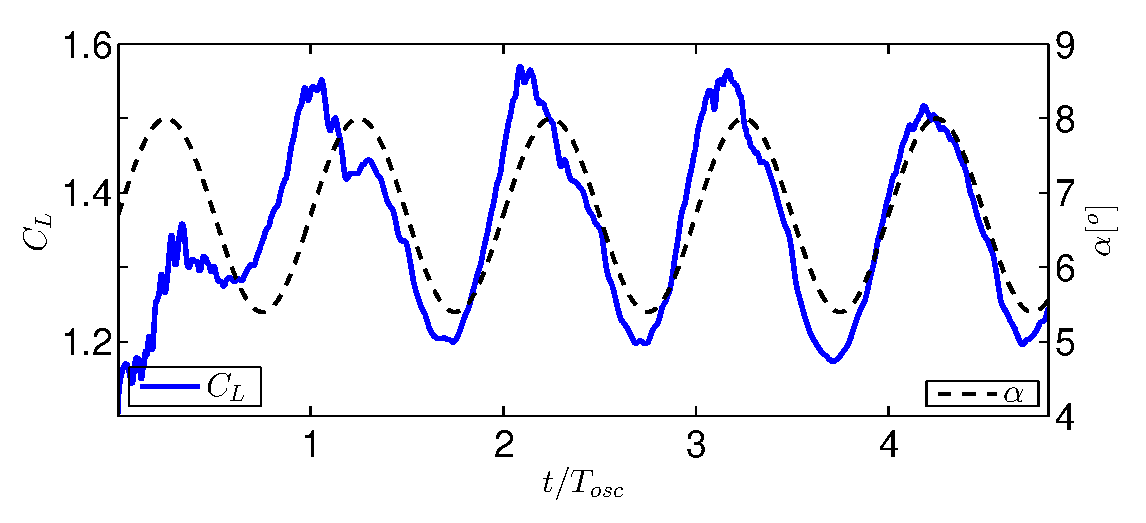
\includegraphics[width=0.85\columnwidth]{cl-time-alpha}
	\caption{Coefficient of Lift ($C_{L} \textcolor{blue}{-}$) and angle of attack $(\alpha \textcolor{black}{--})$ variation with time. $C_{L}$ is on the left axes while $\alpha$ is on the right axes.}
	\label{fig:cl-time-alpha}
\end{figure}

\begin{figure}[h]
	\centering
	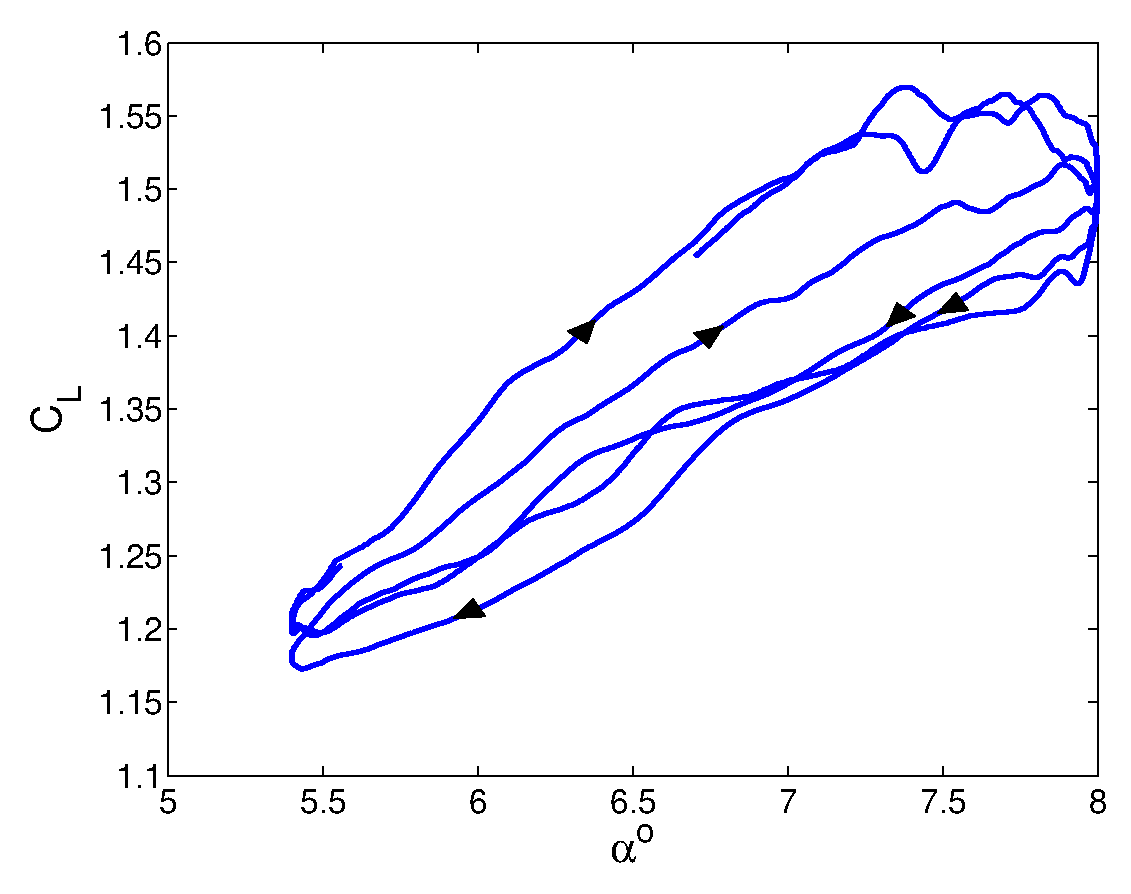
\includegraphics[width=0.85\columnwidth]{cl-alpha}
	\caption{Phase portrait of $C_{L}$ and $\alpha$. The sense of the motion is clockwise, as marked by the arrows.}
	\label{fig:cl-alpha}
\end{figure}

A space-time plot of the instantaneous spanwise averaged wall-shear stress is shown in figure~\ref{fig:cf-time}, which spans the fourth pitch cycle in time. The plot indicates the region of turbulent flow over the airfoil as a function of time. Regions with color intensity strongly towards red show regions of high shear and thus turbulent flow. The exception to the rule being the region close to the leading edge where the flow is laminar but a high shear region exists due to the strong curvature and flow acceleration effects. Inclined streaks of alternating red and blue patterns are signatures of the motion of strong coherent vortices over the airfoil surface, which leave an alternating imprint of positive and negative shear-stress on the wall. These vortices move across the airfoil at a near constant velocity of $U_{vort}\approx0.59$ (marked by the blue arrow in figure~\ref{fig:cf-time}).

Evident from the red colored regions is the abrupt upstream motion of the start of the high shear region just after $t/T_{osc}\approx3.25$, signifying the sharp movement of the transition point. The cause for the sharp transition movement can be found in the instability of the laminar separation bubble (LSB). A phase plot of $C_{L}\ vs\ \alpha$ (figure~\ref{fig:cl-alpha}) for the last two pitch cycles also shows a sudden drop in the integral value which occurs when the pitch cycle is close to the maximum angle of attack.

Regions of separated flow provide an insight into the dynamics of transition and its abrupt motion. Figure~\ref{fig:separation-time} shows the space-time evolution of negative wall-shear stress, marked by the black regions, which are indicative of separated flow. Initially, in the pitch-up phase, no leading edge LSB is present. However vortex rolls can be observed, which create intermittent separation near $x/c\approx0.6$, which is also approximately the start of the high adverse pressure gradient region on the suction side of the airfoil surface. Transition is thus controlled by instability of these vortices. The LSB first appears at $t/T_{osc}=3.14$ during the upward pitch cycle, gradually growing in size and eventually becomes unstable. The LSB instability then becomes the governing mechanism for transition. On the downward cycle ($t/T_{osc}=3.25 - 3.75$) the LSB undergoes the opposite behavior, whereby it ceases to be unstable and slowly shrinks in size to eventually disappear at $t/T_{osc}=3.65$. The turbulent region also visibly detaches from the separation bubble and slowly moves downstream. The airfoil surface thus undergoes a slow relaminarization process. The motion of the boundary between laminar and turbulent regions is indicated by the red arrow in figure~\ref{fig:cf-time}. This downstream motion occurs at a near constant velocity of $U_{lam-turb}\approx0.17$. 
\begin{figure}[h]
	\centering
	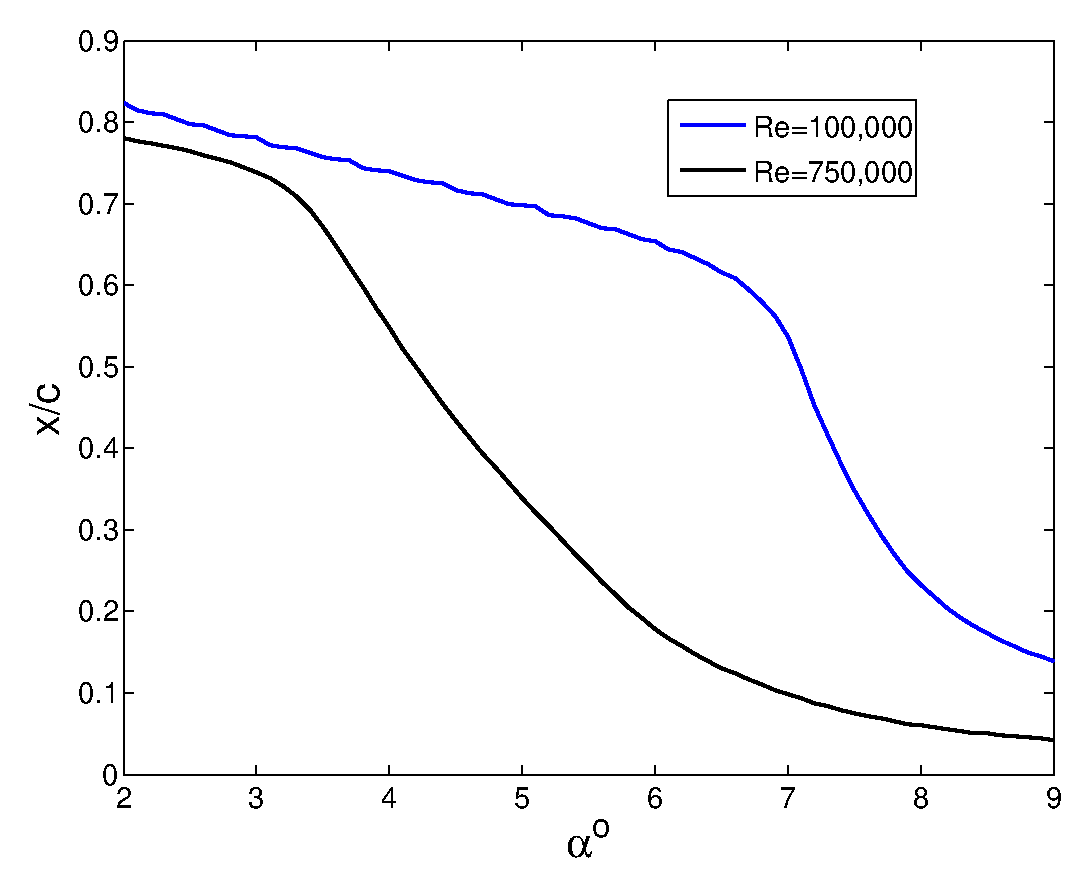
\includegraphics[width=0.75\columnwidth]{tr-xfoil}
	\caption{Reynolds number variation of predicted suction side transition location.}
	\label{fig:tr-xfoil}
\end{figure}
\begin{figure*}
	\centering
	\begin{subfigure}[t]{1\columnwidth}
		\centering
		\includegraphics[width=0.9\columnwidth, height=1\columnwidth]{cf_time_surf}
		\caption{Space-time variation of wall-shear stress ($\tau_{w}$)}. 
		\label{fig:cf-time}
	\end{subfigure}
	\begin{subfigure}[t]{1\columnwidth}
		\centering
		\includegraphics[width=0.8\columnwidth, height=1\columnwidth]{cf_time_surf_grey}
		\caption{Black regions indicate negative wall-shear values} 
		\label{fig:separation-time}
	\end{subfigure}
	\caption{Space-time plot for the wall-shear values ($\tau_{w}$) and separated flow regions. The values are obtained from the instantaneous flow averaged over the spanwise direction. Horizontal blue dashed lines in \ref{fig:separation-time} represent the extremum positions of angle of attack, while the red dashed lines represent phases corresponding to mean angle of attack.}
	\label{fig:space-time}
\end{figure*}

Some insight can be gained on Reynolds number trends from Xfoil, which indicates a large movement of transition location also occurs at higher Reynolds numbers of $Re_{c}=750,000$ (figure~\ref{fig:tr-xfoil}). However at higher Reynolds numbers the separation bubble is expected to be too small to play a significant role. The transition location is then expected to be determined by the instability of Tollmien-Schlichting (TS) waves. However as indicated by the Xfoil data, even the location of TS wave instability changes rapidly with a small $\Delta\alpha$ near $\alpha\approx 3.5^{\circ}$. The effect of pitch oscillations on TS wave instability may again alter the aerodynamic performance of the airfoil.

\section*{SUMMARY AND CONCLUSION}

A relaxation-term filtering procedure is used for wall-resolved LES of flow over a pitching airfoil. The procedure supplements the Navier--Stokes equations with a relaxation term which adds limited high order dissipation in the smallest scales. Validation of the LES procedure is done in a channel flow at $Re_{\tau}=395$ and for a wing section at $Re_{c}=400,000$ and the results show a very good agreement with available DNS data sets.

Flow over a pitching airfoil is simulated using the LES procedure at a chord based Reynolds number of $Re_{c}=100,000$ using an NLF airfoil. The airfoil characteristics exhibit sensitive dependence on angle of attack in certain ``off-design" operating conditions. This predicted sensitive dependence is also captured in the steady simulations at different angles of attack. 

Pitching the airfoil within this $\alpha$ range of sensitive dependence displays a rich variety of unsteady physical phenomena. The flow goes through alternating periods of fully turbulent and laminar flow over the suction side of the airfoil. The point of transition continuously moves across the airfoil surface during the pitch cycles with some rapid upstream movements. On the other hand, relaminarization is a much slower process with the laminar-turbulent boundary moving downstream with a velocity of $U_{lam-turb}\approx0.17$.

Different mechanisms govern the transition point through the different phases of the pitching cycle. In the absence of an unstable LSB and when the suction side surface is mostly laminar, transition is governed primarily by instability of strongly two-dimensional vortices, convecting across the airfoil surface. This remains the governing factor until the appearance of the LSB, which causes a sharp upstream movement of the transition point. The LSB instability is seen to coincide with the end of the pitch-up cycle, and thereafter it remains the governing factor for transition location. On the pitch-down phase, the LSB ceases to be unstable and the transition point then detaches from the separation bubble and slowly moves downstream resulting in a slow relaminarization of airfoil surface.

At higher Reynolds number TS wave instability is expected to be the dominant source of transition to turbulence. However the rapid variation of transition point is still present at higher Reynolds numbers. The response of TS wave transition to small-amplitude pitching remains unknown in such cases where the transition location is highly sensitive. The numerical setup is under way to simulate small-amplitude pitch oscillations at higher Reynolds numbers.

\section*{ACKNOWLEDGEMENT} 

The computations were performed on resources provided by the Swedish National Infrastructure for Computing (SNIC) at the PDC Center for High Performance Computing at the Royal Institute of Technology (KTH). The work was partially funded by European Research Council under grant agreement 694452-TRANSEP-ERC-2015-AdG. The work was also partially funded by Vinnova through the NFFP project UMTAPS, with grant number 2014-00933. We would like to thank Dr. David Eller and Mikaela Lokatt for providing us with the NLF design and the numerous discussions on different aerodynamic aspects of the project.

%%%%%%%%%%%%%%%%%%%%%%%%%%%%%%%%%%%%%%%%%%%%%%%%%%%%%%%%%%%%%%%%%%%%%%
%\FloatBarrier

%%%%%%%%%%%%%%%%%%%%%%%%%%%%%%%%%%%%%%%%%%%%%%%%%%%%%%%%%%%%%%%%%%%%%%
\bibliographystyle{tsfp}
\bibliography{tsfp}
% In this example, BibTeX is used
% For users not familiar with LaTeX, the bibliography can be typed in directly. In this case, comment the two lines above.
%%%%%%%%%%%%%%%%%%%%%%%%%%%%%%%%%%%%%%%%%%%%%%%%%%%%%%%%%%%%%%%%%%%%%%%
%\section*{SAMPLE REFERENCES}
%
%Kwon, O. K., and Pletcher, R. H., 1981, "Prediction of the Incompressible Flow Over a Rearward-Facing Step", Technical Report HTL-26, CFD-4, Iowa State Univ., Ames, IA.
%
%Lee, Y., Korpela, S. A., and Horne, R. N., 1982, "Structure of Multi-Cellular Natural Convection in a Tall Vertical Annulus," Proceedings, 7th International Heat Transfer Conference, U. Grigul et al., ed., Hemisphere Publishing Corp., Washington, D.C., Vol. 2, pp. 221-226.
%
%Sparrow, E. M., 1980a, "Fluid-to-Fluid Conjugate Heat Transfer for a Vertical Pipe - Internal Forced Convection and External Natural Convection", ASME Journal of Heat Transfer, Vol. 102, pp. 402-407.
%
%Sparrow, E. M., 1980b, "Forced-Convection Heat Transfer in a Duct Having Spanwise-Periodic Rectangular Protuberances", Numerical Heat Transfer, Vol. 3, pp. 149- 167.
%
%Tung, C. Y., 1982, Evaporative Heat Transfer in the Contact Line of a Mixture, Ph.D. Thesis, Rensselaer Polytechnic Institute, Troy, NY.

%%%%%%%%%%%%%%%%%%%%%%%%%%%%%%%%%%%%%%%%%%%%%%%%%%%%%%%%%%%%%%%%%%%%%%


\end{document}
